% !TeX spellcheck = en_US
\documentclass[french]{yLectureNote}

\title{Électrocinétique}
\subtitle{Physique}
\author{Paulhenry Saux}
\date{\today}
\yLanguage{Français}

\professor{Allard}%allard@irsamc.ups-tlse.fr
\usepackage{graphicx}%----pour mettre des images
\usepackage[utf8]{inputenc}%---encodage
\usepackage{geometry}%---pour modifier les tailles et mettre a4paper
%\usepackage{awesomebox}%---pour les boites d'exercices, de pbq et de croquis ---d\'esactiv\'e pour les TP de PC
\usepackage{tikz}%---pour deiffner + d\'ependance de chemfig
\usepackage{tkz-tab}
\usepackage{chemfig}%---pour deiffner formules chimiques
\usepackage{chemformula}%---pour les formules chimiques en \'equation : \ch{...}
\usepackage{tabularx}%---pour dimensionner automatiquement les tableaux avec variable X
\usepackage{awesomebox}%---Pour les boites info, danger et autres63
\usepackage{menukeys}%---Pour deiffner les touches de Calculatrice
\usepackage{fancyhdr}%---pour les en-t\^ete personnalis\'ees
\usepackage{blindtext}%---pour les liens
\usepackage{hyperref}%---pour les liens (\`a mettre en dernier)
\usepackage{caption}%---pour la francisation de la l\'egende table vers Tableau
\usepackage{pifont}
\usepackage{array}%---pour les tableaux
\usepackage{lipsum}
\usepackage{yFlatTable}
\usepackage{multicol}
\newcommand{\Lim}[1]{\lim\limits_{\substack{#1}}\:}
\renewcommand{\vec}{\overrightarrow}
\newcommand{\dd}{\mathrm{d}}
\begin{document}
\setcounter{chapter}{3}
\chapter{Circuits du premier ordre}
On souhaite décrire l'évolution du courant ou de la tension dans les circuits (R,C) ou (R,L).
\section{Charge et décharge d'un condensateur dans une résistance}
Le condensateur peut se charger ou se décharger.

On rappelle que $q = CU_C$ et $i=\dot{q}$ et $i=C\dot{U_c}$.
\subsection{Mise en équation de la charge du condensateur}
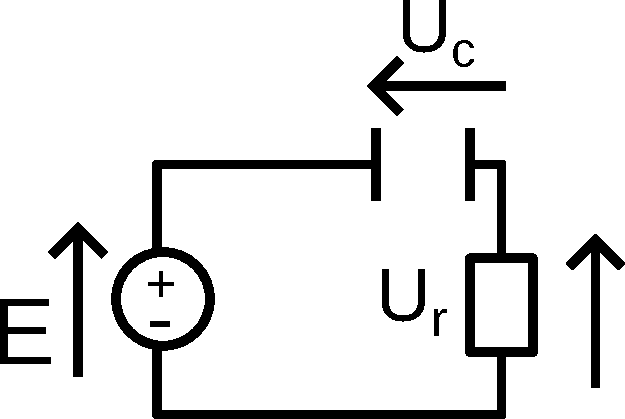
\includegraphics[scale=0.5]{c4-1}

Initialement, le condensateur est déchargé, ses charges et tensions valent 0. À t=0, l'interrupteur passe en position 1. Par la loi des mailles :
\begin{flalign}
E &= U_c+U_R\notag\\
&= U_c +R\times i\notag\\
&= U_c(t)+R\times cU_c(t)'\notag\\
\frac{\dd U_c}{\dd t} + \frac{U_c}{C} &= \frac{E}{\tau}
\end{flalign}
avec \(\tau = RC\).

On résout. La solution générale vaut la solution de l'équation homogène + la solution particulière. Pour la solution  particulière, on cherche une solution de la forme du second membre : \(U^p = B = Cst\). En injectant la constante dans l'équation, on obtient que \(U^p = E\)

On cherche la solution sans second membre telle que \(\frac{\dd U^h_c}{\dd t} + \frac{U^h_c}{C} = 0\). Elle est de la forme \(U^h(t) = Ae^{-t/\tau}\).

Donc \(U_c(t) = E+Ae^{-t/\tau}\). On dit que la constante $A$ est déterminée à partir des conditions initiales, c'est à dire \(U_c(0-) = 0\). Par la propriété de la continuité de la charge aux bornes d'un condensateur, on a \(U_c(0-) = 0 = U_c(0+)\). On en déduit que \(E+A = U_c(0+) = 0 \Rightarrow A = -E\).


\begin{proposition}[Solution d'une équation différentielle d'un condensateur se chargeant]
\[U_c(t) = E(1-e^{-t/\tau})\]
\end{proposition}
Le temps caractéristique est de l'ordre de la miliseconde.

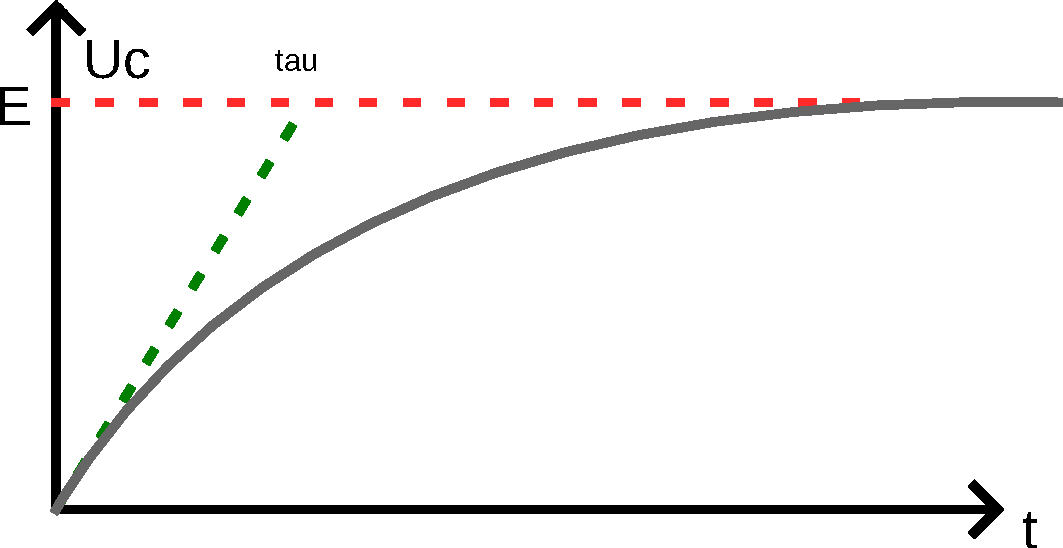
\includegraphics[scale=0.5]{c4-2}
\subsection{Équation de la décharge d'un condensateur}
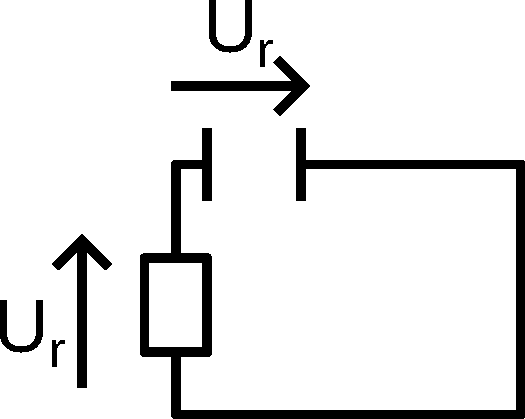
\includegraphics[scale=0.5]{c4-3}

Après un temps long, (le condensateur est chargé sous E), on bascule l'interrupteur en position 2. On part d'une tension qui vaut $E$. On fait décarger le condensateur dans la résistance
\begin{enumerate}
\item On obtient l'équation différentielle par la loi des mailles : \(\frac{\dd U_c}{\dd t} + \frac{1}{\tau} = 0\).
\item On résout \(U_c(t) = A' e^{-t/\tau}\).
\item On détermine A par les conditions initiales : \(U_c(0) = E = A'\).
\end{enumerate}

\begin{proposition}[Solution d'une équation différentielle d'un condensateur se déchargeant]
\[U_c(t) = Ee^{-t/\tau}\]
\end{proposition}
Un condensateur est capable de stocker de l'énergie puis de la restituer sur un temps \(\tau\).

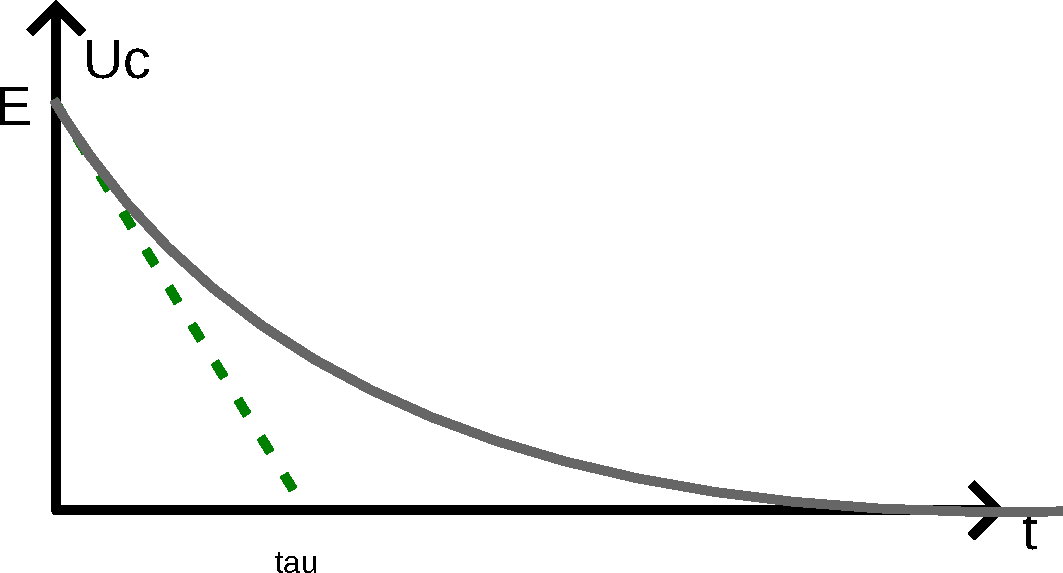
\includegraphics[scale=0.5]{c4-4}
\subsection{Évolution du courant}
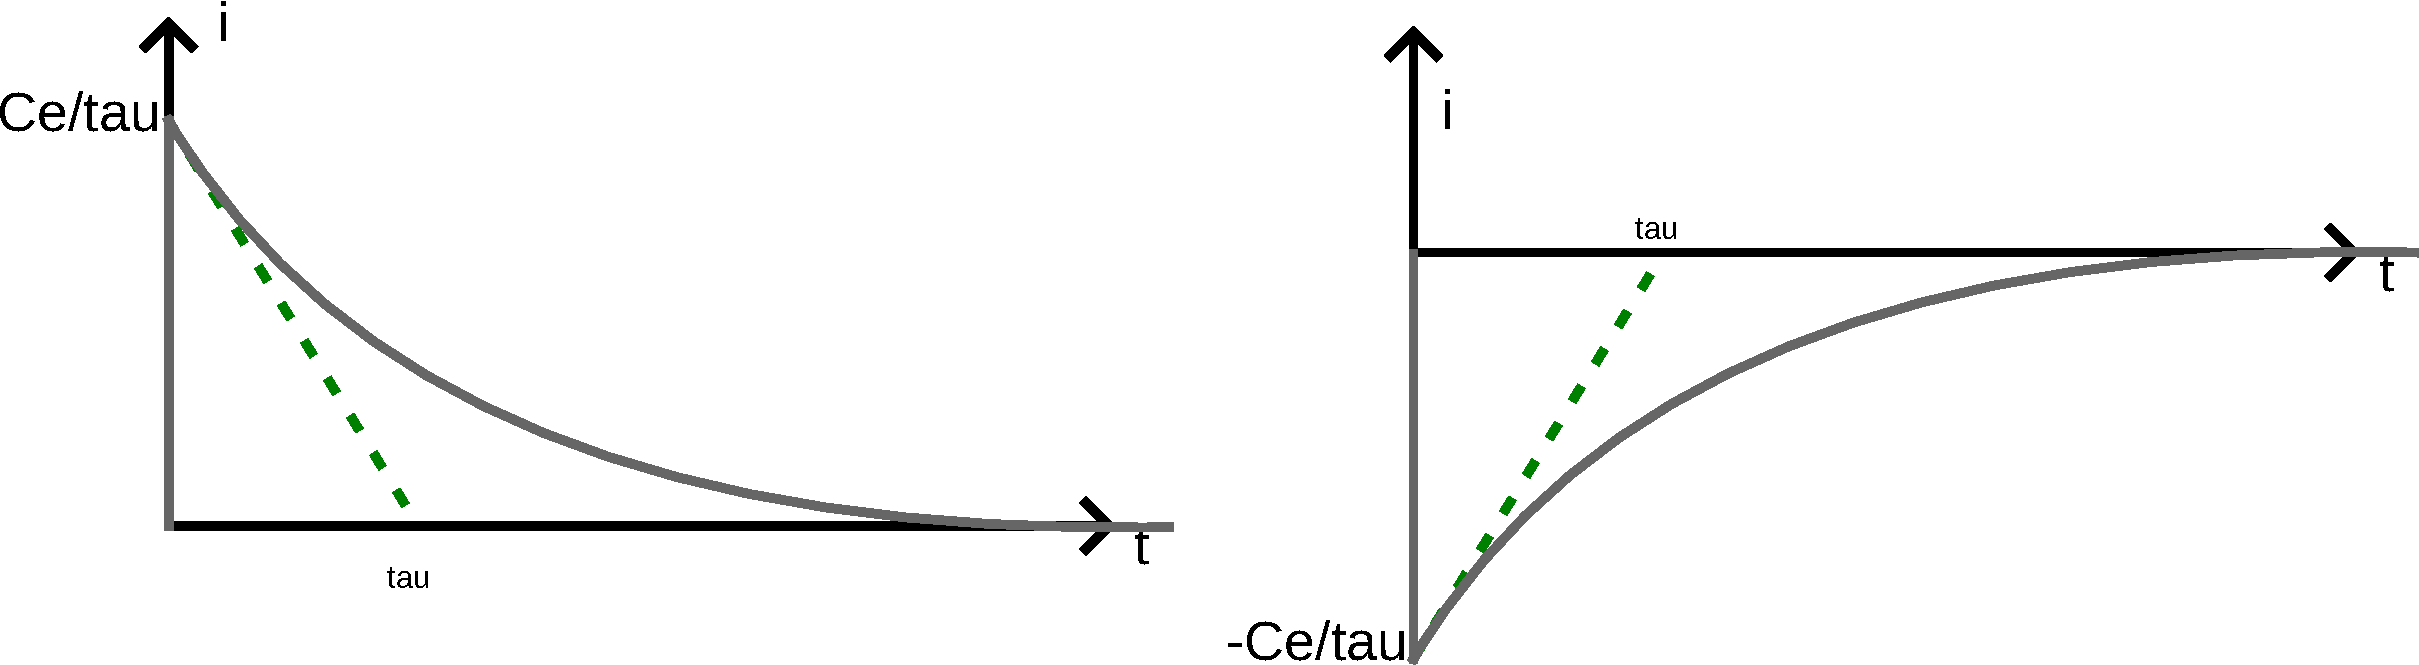
\includegraphics[scale=0.3]{c4-5}
En charge, on a \(U_c(t) = E(1-e^{-t/\tau})\) et en décharge \(U_c(t)\ = Ee^{-t/\tau}\).

On sait aussi que \(i(t) \ = C\frac{\dd U_c}{\dd t}\). En dérivant, on obtient \(i(t) = \frac{CE}{\tau}e^{-t/\tau}\) pour la charge et \(i(t) = -\frac{CE}{\tau}e^{-t/\tau}\) pour la décharge
\warningInfo{Discontinuité du courant}{
Le courant est discontinu dans un condensateur, alors que la tension est bien continue ! Dans une bobine, le courant est par contre continu !}

\section{Circuit RC et régime sinusoidal}
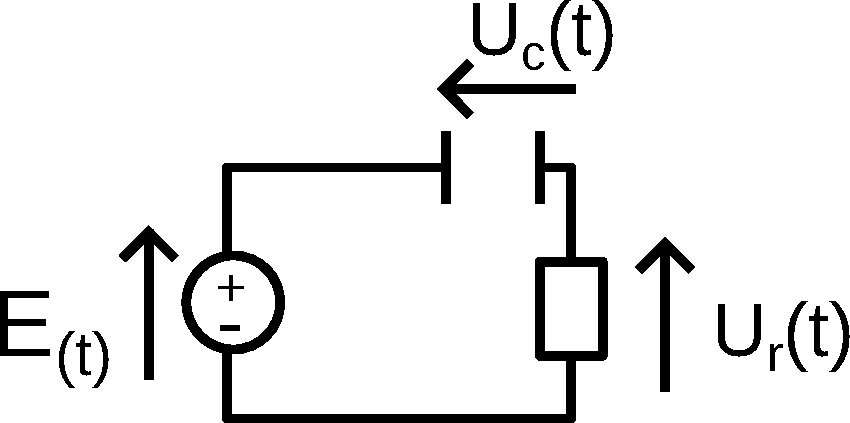
\includegraphics[scale=0.5]{c4-6}
\subsection{Mise en équation}
On a
\begin{flalign}
e(t) &= U_c(t)+U_R(t)\notag\\
&= U_c(t) +R\times i\notag\\
&= U_c(t)+R\times cU_c(t)'\notag\\
\frac{\dd U_c(t)}{\dd t} + \frac{U_c(t)}{C} &= \frac{E_0}{\tau}\cos(\omega t)
\end{flalign}

On trouve la solution homogène : \(Ae^{-t\tau}\)
\subsection{Solution particulière}
Pour la solution particulière, on utilise la méthode de ressemblance, de la forme \(\alpha \cos(\omega t+\varphi)\) ou \({\color{orange}\beta \cos(\omega t) + \gamma \sin(\omega t)}\).

\begin{flalign}
\frac{\dd U_c^p(t)}{\dd t} + \frac{U_c^p(t)}{C} &= -\beta \omega \sin(\omega t)+ \gamma \omega \cos(\omega t)+\frac{1}{\tau}(\beta \cos(\omega t)+\gamma \sin(\omega t))\notag\\
&= (\gamma\omega+\frac{\beta}{\tau})\cos(\omega t)+(\frac{\gamma}{\tau}-\beta \omega)\sin(\omega t)\\
&= \frac{E_0}{\tau} \cos(\omega t)
\end{flalign}
On obtient un système que l'on résout:

\( \left\{\begin{matrix}
\gamma \omega +\frac{\beta}{\tau} &= \frac{E_0}{\tau}\\
\frac{\gamma}{\tau}-\beta \omega &= 0
\end{matrix}\right. \Rightarrow \left\{\begin{matrix}
\gamma &= \frac{E_0}{1+\omega^2\tau^2}\\
\beta &= \frac{E_0\omega \tau}{1+\omega^2\tau^2}
\end{matrix}\right.\)

\subsection{Expression finale}
Donc \(U_c(t) = {\color{red}A e^{-t/\tau}} + {\color{orange}\frac{E_0}{1+\omega^2\tau^2}(\omega \tau \cos(\omega \tau)+\sin(\omega \tau))}\)

On appelle la partie de la solution homogène {\color{red}le régime transitoire} et {\color{orange}l'autre partie }le régime établi.

Pour t supérieur à \(\tau\), après le régime transitoire, toutes les quantités vont suivre l'oscillation sinusoidale du générateur. Il ne reste plus que la{\color{orange} solution paticulière}.

Déterminer la réponse du système en régime établi revient à chercher une {\color{ForestGreen}amplitude} et un {\color{NavyBlue}déphasage} :  \( {\color{ForestGreen}\alpha}\cos(\omega t+{\color{NavyBlue}\varphi})\).
\end{document}

